\begin{table}[H]
\centering
\begin{tabular}{|l|l|l|l|l|}
\hline 
\textbf{Clasificación} & \textbf{Total} & \textbf{Aciertos} & \textbf{Errores} & \textbf{Eficiencia} \\
\hline
Estado & 1393 & 694 & 699 & 49.820 \\
\hline 
Categoría & 1393 & 287 & 1106 & 20.603 \\
\hline 
\end{tabular}
\caption{Eficiencias generales con Hue 40-120}
\label{table:efficiency_general_40_120}
\end{table}

\captionsetup[figure]{skip=-10pt}

\begin{figure}[H]
\centering
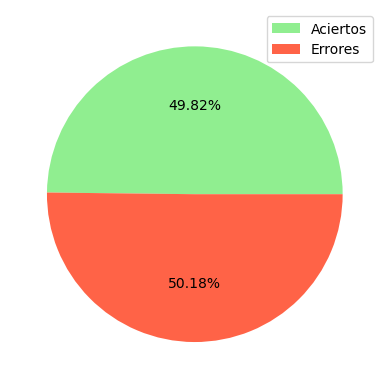
\includegraphics[scale=0.6]{images/result_global_state_40_120.png}
\caption{Eficiencia detectando el estado con Hue 40-120}
\label{img:efficiency_state_40_120}
\end{figure}

\begin{figure}[H]
\centering
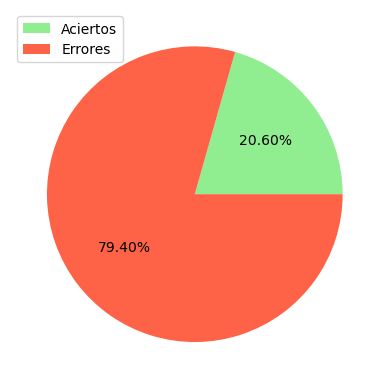
\includegraphics[scale=0.6]{images/result_global_class_40_120.png}
\caption{Eficiencia detectando la categoría con Hue 40-120}
\label{img:efficiency_category_40_120}
\end{figure}

\captionsetup[figure]{skip=10pt}

\begin{table}[H]
\centering
\begin{tabular}{|l|c|c|c|}
\hline 
\textbf{Categoría} & \textbf{Original} & \textbf{Calculado} & \textbf{Eficiencia} \\
\hline
healthy & 791 & 100 & 12.642 \\
\hline 
rust\_level\_1 & 344 & 89 & 25.872 \\
\hline 
rust\_level\_2 & 166 & 69 & 41.566 \\
\hline 
rust\_level\_3 & 62 & 17 & 27.419 \\
\hline 
rust\_level\_4 & 30 & 12 & 40.0 \\
\hline 
\end{tabular}
\caption{Eficiencia por categoría con Hue 40-120}
\label{table:efficiency_categories_40_120}
\end{table}

\begin{figure}[H]
\centering
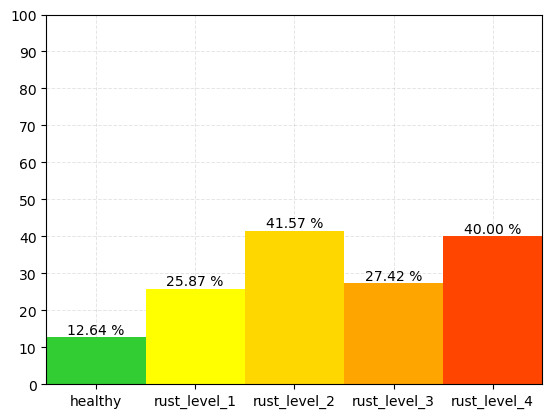
\includegraphics[scale=0.6]{images/result_classes_40_120.png}
\caption{Eficiencia por categoría con Hue 40-120}
\label{img:efficiency_categories_40_120}
\end{figure}
